\setcounter{chapter}{7} 
\chapter*{Chapter (7): Touchscreen Interface}
\addcontentsline{toc}{chapter}{Chapter (7): Touchscreen Interface} 
\renewcommand{\thesection}{\thechapter.\arabic{section}}
\setcounter{section}{0}
\captionsetup[figure]{justification=centering}


\section{Chapter Preview}
This chapter covers the design and implementation of the on-board touchscreen human-machine interface (HMI). It outlines the functional and usability requirements, explains the Preact and Vite technology stack selection, details the application components and WebSocket-based ROS 2 communication, and presents the accessibility design features.

To support these diverse needs, the interface must satisfy a rigorous set of functional and non-functional requirements. The core design principles are simplicity, high visibility, and error-prevention. Since the user may operate the system in motion or under cognitive fatigue, touch targets must be large and forgiving, and system states must be obvious. Table \ref{tab:kiosk-requirements} outlines the system requirements that guided the development of the interface.

\begin{table}[H]
\centering
\caption{Touchscreen Kiosk Interface Functional and Non-Functional Requirements}
\label{tab:kiosk-requirements}
\begin{tabularx}{\textwidth}{|l|>{\raggedright\arraybackslash}X|c|}
\hline
\textbf{Req. ID} & \textbf{Requirement Description} & \textbf{Priority} \\ \hline
FR-01 & Render the local environment map (occupancy grid) in real time. & Must \\ \hline
FR-02 & Allow selecting rooms/saved destinations on the map to trigger Nav2 routing. & Must \\ \hline
FR-03 & Provide a dashboard to view and control connected smart home appliances (lights, AC). & Must \\ \hline
FR-04 & Support hands-free teleoperation of the wheelchair using an eye-gaze dwell system. & Must \\ \hline
FR-05 & Allow manual speed/velocity adjustments and system health diagnostics. & Should \\ \hline
FR-06 & Enable switching between light and dark themes to optimize indoor/outdoor legibility. & Should \\ \hline
FR-07 & Degrade gracefully to an offline/simulation mode if communication with the server is lost. & Must \\ \hline
FR-08 & Support full keyboard and arrow-key navigation for accessibility peripherals. & Must \\ \hline
NFR-01 & Fast startup: First Contentful Paint (FCP) under 1.5 seconds on low-power hardware. & Should \\ \hline
NFR-02 & Lightweight client: Total bundle size under 250 KB when compressed. & Should \\ \hline
NFR-03 & Accessibility compliance: Adhere strictly to WCAG 2.1 Level AA guidelines. & Must \\ \hline
\end{tabularx}
\end{table}

\section{Technology Stack \& Rationale}
Selecting the right software framework for the HMI was critical. The hardware running the interface is a low-power single-board computer (SBC) integrated with the touchscreen panel, meaning resource efficiency is paramount. Heavy modern web application frameworks like React or Electron can introduce high memory overhead and slow startup times, which is unacceptable for an assistive device.

To minimize footprint while maintaining a modular component-driven architecture, \textbf{Preact 10} was chosen as the UI framework. Preact provides the same declarative component model and virtual DOM diffing algorithm as React, but compiles to a runtime of only 3 KB. This results in faster rendering cycles and dramatically lower memory usage. 

\textbf{Vite 7} serves as the build tool and development server, utilizing native ES modules to deliver sub-second hot module replacement (HMR) and optimized build-time tree-shaking. \textbf{Tailwind CSS 4} was selected for styling due to its utility-first class model, which eliminates custom stylesheet bloat and enables rapid implementation of responsive layouts and dark mode states. Finally, the application is written entirely in \textbf{TypeScript 5.9} to ensure compile-time type safety across the ROS 2 message definitions.

Table \ref{tab:framework-comparison} compares the chosen stack with common alternatives evaluated during the design phase.

\begin{table}[H]
\centering
\caption{HMI Technology Stack Comparison}
\label{tab:framework-comparison}
\begin{tabularx}{\textwidth}{|>{\raggedright\arraybackslash}X|c|c|c|c|}
\hline
\textbf{Metric} & \textbf{Preact + Vite} & \textbf{React + CRA} & \textbf{Flutter Web} & \textbf{Electron (App)} \\ \hline
Runtime Core Size & \textasciitilde 3 KB & \textasciitilde 42 KB & \textasciitilde 1.2 MB & \textasciitilde 80 MB \\ \hline
Startup Time (SBC) & < 1.0 s & 2.1 s & 3.5 s & 4.2 s \\ \hline
RAM Consumption & \textasciitilde 18 MB & \textasciitilde 45 MB & \textasciitilde 95 MB & \textasciitilde 160 MB \\ \hline
Touch Interaction & Native & Native & Canvas Emulated & Native \\ \hline
ROS 2 Integration & Direct & Direct & Via Native bridge & Direct \\ \hline
HTML Accessibility & Native ARIA & Native ARIA & Limited & Native ARIA \\ \hline
\end{tabularx}
\end{table}

Key libraries imported into the project (documented in the project's dependencies) include:
\begin{itemize}
    \item \textbf{roslib}: The standard JavaScript library to interface with ROS 2 over a WebSocket connection via \texttt{rosbridge\_suite}.
    \item \textbf{ros2d}: A library built on top of EaselJS that handles 2D visualization of occupancy grid maps and robot poses on an HTML5 canvas.
    \item \textbf{lucide-preact}: A lightweight icon package used to provide descriptive vector symbols for UI controls.
    \item \textbf{clsx} \& \textbf{tailwind-merge}: Utilities to conditionally combine Tailwind classes and eliminate conflicts during dynamic rendering.
\end{itemize}


\section{Application Architecture}
The application codebase is structured according to the clean architecture and SOLID principles. It follows a \textbf{group-by-feature} folder structure to keep code relating to specific functional areas isolated, ensuring composability and separation of concerns.

In \texttt{app.tsx}, the active view is determined by a state variable \texttt{activeTabId}. Rather than unmounting and mounting views dynamically (which would destroy the canvas state and cause expensive re-renders when switching back to the map), the application keeps all panels in the DOM and toggles their visibility using Tailwind's \texttt{hidden} class (compiled as CSS \texttt{display: none}). This technique preserves the WebSocket connection, the occupancy grid canvas representation, and the zoom-and-pan transform matrix, giving the user a seamless and immediate view switch.


\section{ROS 2 Integration \& Service Abstraction}
A critical requirement of the SANAD touchscreen HMI is its ability to interface with multiple backends depending on the environment. When the kiosk runs directly on the wheelchair's onboard computer, it interfaces directly with ROS 2 via WebSockets. When deployed as a remote web interface, it speaks to an intermediate Node.js server. During development or offline testing, it can run entirely client-side using local simulations.

To support this without duplicating UI code, a strict \textbf{Service Abstraction Layer} was implemented using the Factory design pattern. Every business feature defines an interface (e.g., \texttt{IMapService}, \texttt{IRoomService}, \texttt{ISmartHomeService}, and \texttt{IWheelchairService}) that has three distinct implementations:
\begin{itemize}
    \item \textbf{Native Service}: Operates directly over ROS 2 topics and actions using the browser's WebSocket connected to the robot's \texttt{rosbridge\_server}.
    \item \textbf{Server Service}: Sends HTTP REST commands and registers server-sent event (SSE) listeners pointing to the intermediate Node.js server.
    \item \textbf{Simulation Service}: Uses simulated in-memory timers, local storage registries, and coordinate offsets to mimic robot feedback without real hardware.
\end{itemize}

The connection mode is determined by the application's environment configuration. Table \ref{tab:connection-modes} shows how these modes resolve at runtime.

\begin{table}[H]
\centering
\caption{HMI Service Connection Modes}
\label{tab:connection-modes}
\begin{tabularx}{\textwidth}{|l|l|>{\raggedright\arraybackslash}X|>{\raggedright\arraybackslash}X|}
\hline
\textbf{Mode} & \textbf{Protocol} & \textbf{Target Backend} & \textbf{Typical Use Case} \\ \hline
\texttt{NATIVE} & WebSocket & Local ROS 2 Bridge & Running locally on the onboard SBC \\ \hline
\texttt{SERVER} & HTTP REST & Node.js Remote Server & Caregiver monitoring via tablet \\ \hline
\texttt{SIMULATION} & In-Memory & Web Browser Sandbox & Demo booths, UI design, offline testing \\ \hline
\end{tabularx}
\end{table}

The resolution of the active service class is handled by factory singletons. For example, \texttt{MapServiceFactory.getService()} resolves to the appropriate service implementation based on the active connection type and the network status. If a connection exception occurs, the factory can update the local server health state to offline to prevent the UI from locking up or crashing, providing a safe, predictable user experience.

\section{Touchscreen-to-Server Communication Architecture}
The touchscreen kiosk interface functions as the central HMI (Human-Machine Interface) of the SANAD wheelchair system. To ensure that the user interface remains lightweight and responsive, and to prevent tight coupling between core robotic control systems and presentation components, all external interactions are mediated by a supervisory Node.js backend server. This section details the dual-channel communication architecture, data flow protocols, state synchronization mechanisms, and connection resiliency frameworks that govern the interface between the touchscreen client and the supervisory server.

\subsection{Communication Topology}
The communication layout consists of three primary layers: the presentation layer running on the client browser (Preact HMI), the supervisory layer running on the onboard single-board computer (Node.js backend), and the control/execution layer (ROS 2 navigation stack and IoT smart home peripherals). Figure \ref{fig:hmi-server-comm-tikz} illustrates the network topology and the dual-channel transport mechanisms connecting these layers.

\begin{figure}[H]
\centering
\begin{tikzpicture}[
    font=\sffamily\small,
    node distance=2.0cm and 2.2cm,
    clientNode/.style={rectangle, draw=blue!70!black, fill=blue!10, rounded corners, minimum width=3.5cm, minimum height=1.2cm, align=center, thick, drop shadow},
    serverNode/.style={rectangle, draw=orange!80!black, fill=orange!10, rounded corners, minimum width=3.5cm, minimum height=1.2cm, align=center, thick, drop shadow},
    hardwareNode/.style={rectangle, draw=green!60!black, fill=green!10, rounded corners, minimum width=3.5cm, minimum height=1.2cm, align=center, thick, drop shadow},
    peripheralNode/.style={rectangle, draw=purple!70!black, fill=purple!10, rounded corners, minimum width=3.5cm, minimum height=1.2cm, align=center, thick, drop shadow},
    httpArrow/.style={Latex-Latex, draw=red!70!black, thick},
    wsArrow/.style={Latex-Latex, draw=teal!70!black, dashed, thick},
    rosArrow/.style={Latex-Latex, draw=green!60!black, thick},
    udpArrow/.style={-Latex, draw=purple!70!black, thick}
]

    \node[clientNode] (hmi) {Touchscreen HMI\\(Preact Frontend)};
    
    \node[serverNode, right=of hmi, yshift=1cm] (express) {Node.js REST API\\(Aggregator \& JWT)};
    \node[serverNode, right=of hmi, yshift=-1cm] (wsServer) {WebSocket Server\\(Telemetry \& Control)};
    
    \node[hardwareNode, right=of wsServer] (rosbridge) {ROS 2 Bridge\\(rosbridge\_server)};
    \node[peripheralNode, right=of express] (iot) {Smart Home Devices\\(IoT Peripherals)};
    
    \node[hardwareNode, below=of rosbridge] (ros) {ROS 2 Navigation\\(Nav2 / SLAM)};

    \begin{scope}[on background layer]
        \node[draw=orange!60, fill=orange!5, dotted, thick, rounded corners, fit=(express) (wsServer), label={[orange!80!black]above:Node.js Backend Server}] (serverGroup) {};
    \end{scope}

    \draw[httpArrow] (hmi) -- node[above, sloped, font=\tiny] {HTTPS REST (JWT)} (express);
    \draw[wsArrow] (hmi) -- node[below, sloped, font=\tiny] {WS persistent} (wsServer);
    
    \draw[rosArrow] (wsServer) -- node[above, font=\tiny] {JSON over WS} (rosbridge);
    \draw[rosArrow] (rosbridge) -- node[right, font=\tiny] {Native ROS 2} (ros);
    \draw[udpArrow] (express) -- node[above, font=\tiny] {UDP Broadcast} (iot);

\end{tikzpicture}
\caption{Communication topology showing the dual transport paths (REST and WebSockets) between the Preact HMI, the Node.js server wrapper, and the robotic/IoT backends.}
\label{fig:hmi-server-comm-tikz}
\end{figure}

\subsection{Dual-Channel Transport Protocol}
The connection between the touchscreen client and the server leverages two distinct network protocols to optimize for different data transmission requirements:
\begin{itemize}
    \item \textbf{RESTful API Channel (Stateless HTTP/HTTPS)}: This channel is reserved for transactional, low-frequency control actions and query requests. Actions such as requesting a list of pre-configured rooms and coordinate goals, saving user network preferences, and invoking local network discovery scans for smart home devices are conducted via HTTP. To secure this channel, each request must include a signed JSON Web Token (JWT) in its authorization header. Payload verification is enforced on the server prior to controller execution, ensuring that only authenticated, properly formatted requests are processed.
    \item \textbf{WebSocket Channel (Persistent Duplex TCP)}: Real-time control and environmental updates require a low-latency, bidirectional data flow that cannot be efficiently sustained via request-response polling. A persistent WebSocket connection is established between the touchscreen and the server. This channel continuously transmits the wheelchair's telemetry state, occupancy grid update frames, robot position coordinates, and real-time linear/angular teleoperation velocity commands. By bypassing the overhead of standard HTTP handshakes and headers, this persistent socket minimizes latency, ensuring immediate responsiveness during gaze-control driving or manual navigation overrides.
\end{itemize}

\subsection{Serialization and Type Verification}
Data transmitted over both REST and WebSocket channels is structured using lightweight JavaScript Object Notation (JSON). In order to maintain system integrity, data contracts are defined on both ends. The client-side Preact application enforces structural validation using TypeScript types, while the server verifies incoming payloads against predefined schemas before routing them to the ROS 2 integration layer. This bidirectional verification ensures that malformed inputs, such as negative temperature bounds or out-of-range navigation coordinates, are intercepted and rejected at the application boundary, protecting the physical actuators from erratic signals.

\subsection{State Synchronization and Conflict Resolution}
The HMI client maintains local variables representing the status of connected devices (e.g. lighting states, active speed profiles, and active navigation goals). To keep the user interface consistent with the physical world, the system adopts an optimistic UI update model:
\begin{itemize}
    \item When a user changes a setting, such as turning off a smart light, the touchscreen UI immediately reflects the new state.
    \item The client issues an asynchronous HTTP command to the Node.js server.
    \item If the command fails (due to database lock or network disruption), the client captures the error, reverts the local state, and prompts the user with an error notification.
    \item System-critical parameters, including network configurations and current active themes, are persisted locally using the client browser's storage API, allowing the touchscreen HMI to re-initialize to its last known safe state immediately upon reboot.
\end{itemize}

\subsection{Connection Resiliency and Error Recovery}
Given that the touchscreen and the server communicate over local Wi-Fi or internal virtual networks, connection drops can occur. To prevent erratic behaviors, the system implements a robust connection lifecycle manager:
\begin{itemize}
    \item \textbf{Heartbeat Monitor}: The client and server exchange small keep-alive frames at regular intervals. If the client fails to receive a ping acknowledgement within $1500\text{ ms}$, the connection is flagged as degraded.
    \item \textbf{Safe Degradation}: Upon detecting a connection drop, the touchscreen interface automatically displays a prominent red warning banner and locks out manual drive commands, preventing the user from issuing steering requests while the state is uncertain.
    \item \textbf{Reconnection Strategy}: The client initiates a reconnection loop using exponential backoff.
    \item \textbf{Hardware Fail-Safe}: To ensure safety during teleoperation, the underlying ROS 2 velocity controller monitors the keep-alive signal. If no velocity update command is received from the HMI over the WebSocket channel within $500\text{ ms}$, the motor driver automatically halts the wheelchair, preventing runaway collisions in the event of an HMI crash or network failure.
\end{itemize}

\section{Home Dashboard}
The first view presented to the user is the Home Dashboard, implemented in \texttt{HomeView.tsx}. It serves as a visual launcher, providing a clean, distraction-free grid containing four high-contrast touch cards.

The primary functions displayed are:
\begin{itemize}
    \item \textbf{Map Navigation}: Navigates the user to the interactive map viewport for route visualization and destination selection.
    \item \textbf{Hands-Free Control}: Opens the radial eye-tracking interface, allowing users with severe paralysis to drive the chair or operate the home.
    \item \textbf{Smart Home}: Displays a dedicated grid for IoT smart appliance management.
    \item \textbf{System Settings}: Grants access to theme adjustments, notifications, and bridge endpoints.
\end{itemize}

The layout uses a two-column, two-row responsive grid with rounded panels (\texttt{rounded-2xl}), subtle gradients, and prominent SVG icons. The design is optimized for low visual clutter to ensure readability under varying light conditions.

\begin{figure}[H]
\centering
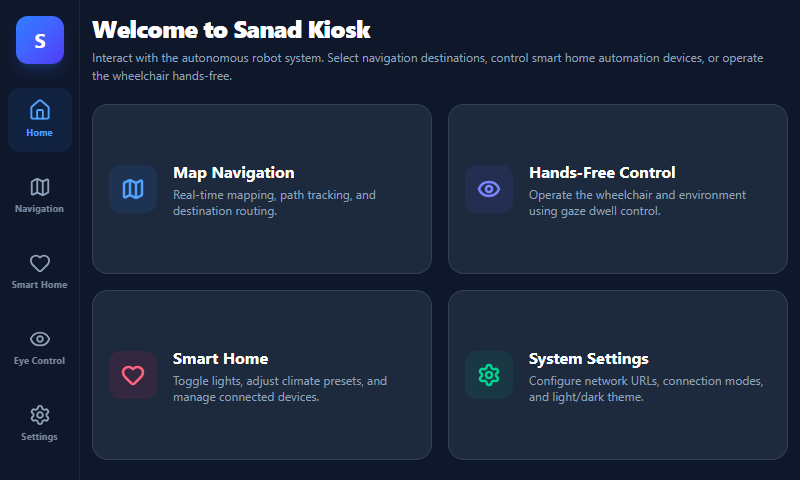
\includegraphics[width=0.6\textwidth]{figures/ch07/home_dark.png}
\caption{Home Dashboard UI in Dark Mode showing the high-contrast button grid.}
\label{fig:home-dark}
\end{figure}

\section{Real-Time Map \& Navigation Interface}
The map interface (\texttt{MapView.tsx}) is the most complex module in the touchscreen package. It integrates a 2D rendering pipeline to present an occupancy grid map constructed by the SLAM (Simultaneous Localization and Mapping) perception stack.

\subsection{Occupancy Grid Model}
The map data is received as a ROS message containing the map metadata and cell weights:
\begin{equation}
M = \{H, I, D\}
\end{equation}
where $H$ is the header containing coordinate frame references and stamps, $I$ is the map metadata (resolution, grid width, grid height, and origin pose), and $D$ is a one-dimensional array of occupancy probability values:
\begin{equation}
d_i \in [-1, 0, \dots, 100]
\end{equation}
where $-1$ represents an unexplored cell, $0$ is free space, and $100$ is a confirmed obstacle.

\subsection{Map Rendering Canvas}
In \texttt{MapCanvas.tsx}, the occupancy grid data is read and parsed. A canvas rendering pipeline translates the 1D array into an image bitmap using offscreen canvas buffers. The resolution of the map (typically $0.05$ meters/pixel) is used to draw the boundary walls, corridors, and obstacle points.
A custom coordinate transformation handles mapping between the ROS world coordinate frame (origin at center of SLAM mapping) and the local HTML5 canvas coordinate frame (origin at top-left, measured in pixels):
\begin{align}
x_{\text{canvas}} &= \frac{x_{\text{world}} - x_{\text{origin}}}{\text{resolution}} \\
y_{\text{canvas}} &= \text{height}_{\text{grid}} - \frac{y_{\text{world}} - y_{\text{origin}}}{\text{resolution}}
\end{align}

\subsection{Robot Pose \& Navigation Control}
The robot's current position and heading ($x, y, \theta$) are retrieved from the coordinate transform tree (\texttt{/tf}) and rendered as a custom oriented triangle icon on top of the map. 
The user can navigate the wheelchair in two ways:
\begin{itemize}
    \item \textbf{Tap-to-Goal}: Clicking anywhere on the map canvas triggers a callback that translates the canvas pixel coordinates back to a ROS pose. This coordinates are sent to the Nav2 Action Server as a new navigation goal.
    \item \textbf{Quick Navigation Sidebar}: A drawer list displaying saved destinations (e.g., "Bedroom", "Kitchen", "Living Room"). Tapping a destination sends the pre-registered coordinates of that room.
\end{itemize}

During navigation, a dedicated status card displays feedback retrieved from the Action Server, including the remaining distance in meters, the estimated time remaining in seconds (ETA), and recovery behaviors triggered. A cancel button is available to halt autonomous motion immediately.

\begin{figure}[H]
\centering
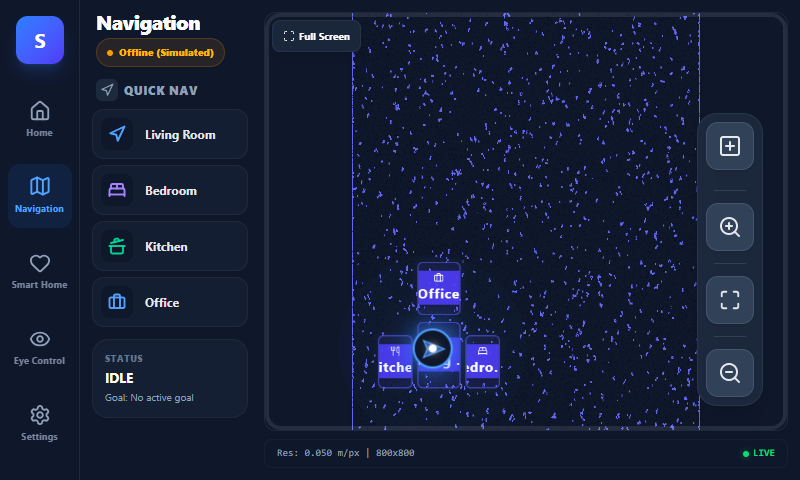
\includegraphics[width=0.9\textwidth]{figures/ch07/map_overview.png}
\caption{Map Viewport showing the 2D occupancy grid, registered rooms, and the Quick Navigation sidebar panel.}
\label{fig:map-overview}
\end{figure}

\section{Smart Home Control Panel}
The smart home integration interface (\texttt{SmartHomeView.tsx}) allows users to control IoT appliances in their home directly from the wheelchair touchscreen. It communicates with the intermediate Node.js server to monitor and control devices.

\subsection{Device Discovery}
By tapping the "Scan Network" button, the HMI triggers a network-wide discovery protocol. The server sends a UDP broadcast command on the local subnet to detect active smart appliances. Discovered devices are returned as an array, including their unique hardware ID, name, IP address, control type, and current state.

\subsection{Device Organization \& Control Widgets}
The application automatically categorizes discovered devices based on name and category metadata, grouping them into five clear visual sections: Lighting, Climate, Security, Media, and Other.
Each device category maps to a specialized control widget, as defined in Table \ref{tab:smart-home-controls}.

\begin{table}[H]
\centering
\caption{Smart Home Device Control Widgets}
\label{tab:smart-home-controls}
\begin{tabularx}{\textwidth}{|l|l|>{\raggedright\arraybackslash}X|l|}
\hline
\textbf{Device Type} & \textbf{Control Type} & \textbf{UI Widget Used} & \textbf{Example Commands} \\ \hline
Smart Light & \texttt{toggle} & Sliding toggle switch & \texttt{turn\_on} / \texttt{turn\_off} \\ \hline
Air Conditioner & \texttt{slider} & Horizontal range input slider (0--30) & \texttt{set\_temperature} (Celsius) \\ \hline
Media / TV & \texttt{toggle} & Sliding toggle switch & \texttt{power\_on} / \texttt{power\_off} \\ \hline
Door Lock & \texttt{button} & Instant click action button & \texttt{lock} / \texttt{unlock} \\ \hline
Dimmer Switch & \texttt{slider} & Horizontal range input slider (0--100) & \texttt{set\_brightness} \\ \hline
\end{tabularx}
\end{table}

\begin{figure}[H]
\centering
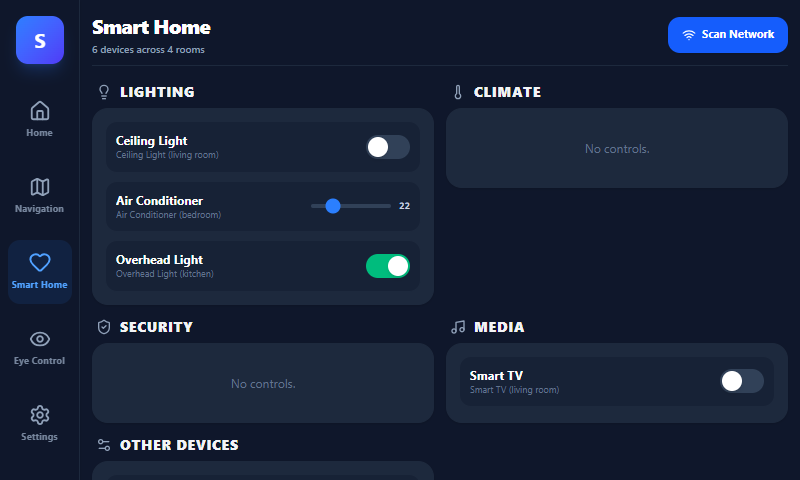
\includegraphics[width=0.9\textwidth]{figures/ch07/smarthome_panel.png}
\caption{Smart Home control panel showing active device controls grouped into Lighting, Climate, and Media sections.}
\label{fig:smarthome-panel}
\end{figure}

\section{Eye Tracking Interface \& Gaze Dwell}
For users with quadriplegia or advanced neuromuscular disorders (such as Amyotrophic Lateral Sclerosis or Multiple Sclerosis), standard physical touch control is not possible. For these users, the touchscreen serves as the primary visual display for an \textbf{Eye Tracking Interface} (\texttt{EyeControlView.tsx}). The hardware details of the physical infrared gaze cameras are discussed in later chapters; this section focuses on the software implementation of the radial gaze-wheel layout and the dwell-selection algorithm.

\subsection{Gaze Wheel Menu System}
The gaze interface is built as a radial menu (\texttt{GazeWheel.tsx}). Traditional grids are difficult for eye tracking because the gaze points can drift, leading to accidental selection of adjacent cells. A circular menu divides the screen into large pie-slice sectors around a central neutral region. This layout maximizes the distance between selectable areas, improving reliability.

The radial menu is hierarchical:
\begin{itemize}
    \item \textbf{Main Menu}: Displays top-level categories, including Navigation, Toggle Lights, Thermostat, Media, Door Locks, Wheelchair Drive, and Dwell Settings.
    \item \textbf{Sub-Menu - Navigation}: Dynamically lists registered rooms (e.g. Living Room, Bedroom) derived from \texttt{useRooms.ts}.
    \item \textbf{Sub-Menu - Wheelchair}: Displays motor commands: Forward, Turn Left, Stop, Turn Right, and Backward.
    \item \textbf{Sub-Menu - Dwell Settings}: Allows adjusting the validation timer to match the user's calibration quality.
\end{itemize}

\subsection{Gaze Dwell Selection Algorithm}
To register a select action without a physical click, the software uses a \textbf{gaze dwell mechanism} (\texttt{useGazeDwell.ts}). When the eye tracker detects the user's focus on a specific sector, a validation timer begins.
Let $S_i$ be the targeted sector, and $t_{\text{hover}}$ be the continuous duration the gaze remains within the sector boundary. The progress fraction $P(S_i)$ is computed at $30\text{ ms}$ intervals:
\begin{equation}
P(S_i) = \min\left(1, \frac{t_{\text{hover}}}{T_{\text{dwell}}}\right)
\end{equation}
where $T_{\text{dwell}}$ is the configurable dwell time selected by the user. 
Visually, this progress is rendered as a circular progress ring drawing around the sector. If $P(S_i) \geq 1.0$, the selection is confirmed, the action callback is fired, and the interface triggers a brief visual flash.
To prevent accidental repeated activations (the "Midas touch" problem), a cooldown state is immediately entered:
\begin{equation}
t_{\text{cooldown}} = 600\text{ ms}
\end{equation}
During this period, all selections are locked out. If the user's gaze drifts out of the sector at any point before $P(S_i) = 1.0$, the timer is cleared and the progress resets to $0$. 

\begin{figure}[H]
\centering
\begin{tikzpicture}[
    font=\sffamily\small,
    node distance=2.2cm and 2.5cm,
    state/.style={circle, draw=teal!80!black, fill=teal!10, thick, minimum size=2.2cm, align=center, drop shadow},
    triggerState/.style={circle, draw=orange!80!black, fill=orange!10, thick, minimum size=2.2cm, align=center, double, drop shadow},
    arrow/.style={-Latex, thick, draw=gray!80},
    transLabel/.style={font=\tiny, fill=white, align=center}
]

    % States
    \node[state] (idle) {Idle\\($P = 0$)};
    \node[state, right=of idle] (hover) {Gaze Hovering\\($P < 1.0$)};
    \node[triggerState, right=of hover] (selected) {Action Selected\\($P \ge 1.0$)};
    \node[state, below=of hover] (cooldown) {Cooldown\\($t_{\text{cooldown}} < 600\text{ ms}$)};

    % Transitions
    \draw[arrow] (idle) -- node[above, transLabel] {Gaze Enters\\Sector} (hover);
    \draw[arrow] (hover) -- node[above, transLabel] {Timer Expires\\($t_{\text{hover}} \ge T_{\text{dwell}}$)} (selected);
    
    % Hover to Idle (Reset)
    \draw[arrow, bend right=30] (hover) to node[below, transLabel] {Gaze Leaves\\Sector} (idle);
    
    % Selected to Cooldown
    \draw[arrow] (selected) |- node[below right, transLabel] {Trigger Callback\\(Flash UI)} (cooldown);
    
    % Cooldown to Idle
    \draw[arrow] (cooldown) -| node[below left, transLabel] {Cooldown Expires\\($t > 600\text{ ms}$)} (idle);

\end{tikzpicture}
\caption{State machine diagram illustrating the gaze-dwell selection and error-prevention lifecycle.}
\label{fig:gaze-dwell-state-machine}
\end{figure}

\begin{figure}[H]
\centering
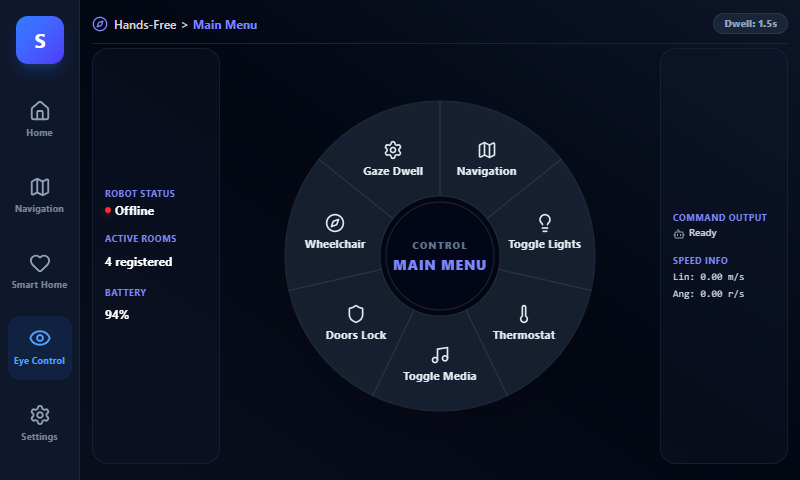
\includegraphics[width=0.7\textwidth]{figures/ch07/gaze_wheel_main.png}
\caption{Main Menu of the hands-free gaze interface, showing the radial layout and central "neutral" sector.}
\label{fig:gaze-wheel-main}
\end{figure}

\section{Wheelchair Teleoperation Interface}
For users operating the wheelchair through alternative controllers or direct screen interaction, a software \textbf{Wheelchair Teleoperation Mode} is integrated. In this mode, the client sends velocity commands directly to the robot.

The wheelchair's target velocity command is defined by the linear velocity $v$ and angular velocity $\omega$:
\begin{align}
v &\in [-1.0, 1.0]\text{ m/s} \quad \text{(normalized)} \\
\omega &\in [-1.0, 1.0]\text{ rad/s} \quad \text{(normalized)}
\end{align}
These inputs are sent via the \texttt{updateVelocity(linear, angular)} function in \texttt{IWheelchairService}.
When using the eye-control drive sub-wheel, the directional commands map to pre-configured safe velocity thresholds:
\begin{itemize}
    \item \textbf{Move Forward}: $v = 0.3\text{ m/s}, \omega = 0.0\text{ rad/s}$
    \item \textbf{Turn Left}: $v = 0.0\text{ m/s}, \omega = 0.4\text{ rad/s}$
    \item \textbf{Turn Right}: $v = 0.0\text{ m/s}, \omega = -0.4\text{ rad/s}$
    \item \textbf{Move Backward}: $v = -0.3\text{ m/s}, \omega = 0.0\text{ rad/s}$
    \item \textbf{STOP}: $v = 0.0\text{ m/s}, \omega = 0.0\text{ rad/s}$
\end{itemize}



Safety is a primary design consideration. In addition to the physical emergency stop switches, a software safety stop is always visible as a red octagon in the center of the driving sub-wheel. Additionally, the wheelchair controller automatically times out and halts the motors if it does not receive a keep-alive velocity command within $500\text{ ms}$.

\section{Settings \& Configuration Management}
The settings view (\texttt{SettingsView.tsx}) manages user preferences and interface parameters.
It is divided into three sections:
\begin{itemize}
    \item \textbf{Appearance}: Allows selecting the display theme (Light, Dark, or System Sync).
    \item \textbf{Connection}: Configures the backend integration mode (NATIVE, SERVER, or SIMULATION) and allows overriding WebSocket/REST API URLs to adapt to local networks.
    \item \textbf{Notifications}: Toggles desktop and audio alerts for obstacle warnings and connection losses.
\end{itemize}

All configuration parameters are stored locally on the client device using the browser's \texttt{localStorage} API. This ensures settings persist across system reboots. To ensure clean state initialization, saving new connection parameters resets the health flag and refreshes the browser window using \texttt{window.location.reload()}, which re-initializes all factories and initiates clean WebSocket connections to the new endpoints.

\begin{figure}[H]
\centering
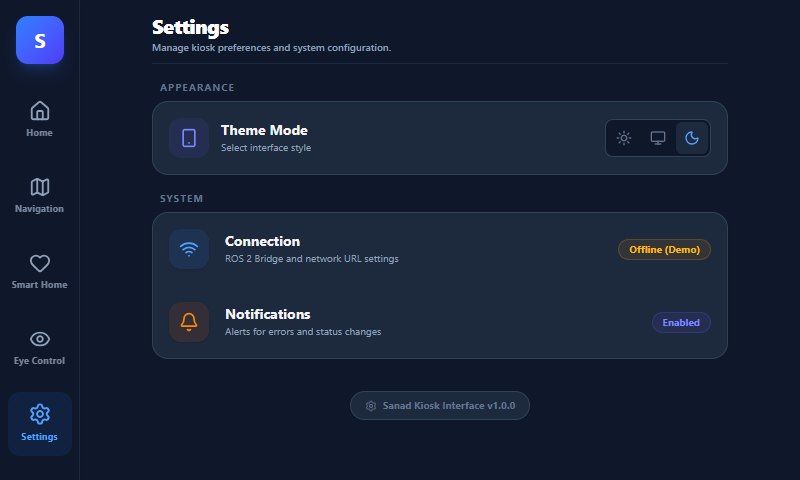
\includegraphics[width=0.7\textwidth]{figures/ch07/settings_overview.png}
\caption{Settings view showing configuration options for themes, network endpoints, and system parameters.}
\label{fig:settings-overview}
\end{figure}

\section{Accessibility Design}
Providing full access to users with motor impairments requires strict adherence to web accessibility guidelines (WCAG 2.1 Level AA).

\subsection{ARIA Attributes \& Semantics}
The interface uses semantic HTML structure and ARIA (Accessible Rich Internet Applications) attributes to support screen readers and switch-access devices. 
Table \ref{tab:accessibility-aria} lists the ARIA patterns used in the interface.

\begin{table}[H]
\centering
\caption{Application ARIA Accessibility Patterns}
\label{tab:accessibility-aria}
\begin{tabularx}{\textwidth}{|l|>{\raggedright\arraybackslash}X|>{\raggedright\arraybackslash}X|>{\raggedright\arraybackslash}X|}
\hline
\textbf{Pattern} & \textbf{ARIA Attributes} & \textbf{Target Element} & \textbf{Usage Rationale} \\ \hline
Tab Control & \texttt{role="tablist"}, \texttt{role="tab"} & Sidebar navigation buttons & Represents the primary application sections. \\ \hline
Tab Panel & \texttt{role="tabpanel"} & Core viewport frames & Links each panel container to its corresponding tab button. \\ \hline
Selection State & \texttt{aria-selected="true"} & Active tab element & Identifies the currently selected view. \\ \hline
Control State & \texttt{aria-checked="true"} & Selected radio button & Indicates the active option (e.g. active theme). \\ \hline
Grid Lists & \texttt{role="list"}, \texttt{role="listitem"} & Home menu dashboard buttons & Groups launch shortcuts into structured groups. \\ \hline
Labels & \texttt{aria-label="string"} & Custom icon-only buttons & Provides clear descriptions for controls without text labels. \\ \hline
\end{tabularx}
\end{table}

\subsection{Keyboard \& Arrow Key Navigation Hook}
To accommodate mechanical switches (such as sip-and-puff controls or head-rest switches) that mimic standard keyboard events, a custom navigation hook was developed (\texttt{useArrowNavigation.ts}).
This hook captures keyboard focus events within containers (like \texttt{role="tablist"} or \texttt{role="list"} grids). When an arrow key is pressed, the hook intercepts the default browser event, computes the target element's index, and moves focus programmatically. This allows full control over the application's tabs, buttons, sliders, and modal dialogs using only four keyboard events (or a single scanning switch). Focus indicators are styled with highly visible borders (\texttt{focus-visible:ring-4}) to assist users with visual impairments.

\section{Dark Mode \& Theming System}
To ensure the interface is readable in different environments (such as direct sunlight or dark rooms), the application features a persistent theming system (\texttt{useTheme.ts}). 

The theme can be set to:
\begin{itemize}
    \item \textbf{Light Mode}: Optimizes contrast for bright outdoor environments, using slate-colored text against a pure white background.
    \item \textbf{Dark Mode}: Reduces glare and eye strain in dim indoor settings, using white text against a deep slate background.
    \item \textbf{System Mode}: Syncs the app theme with the operating system's setting using a CSS media query.
\end{itemize}

The theme is applied by adding the \texttt{"dark"} class to the root HTML element, enabling Tailwind's \texttt{dark:} styling variants for all components. Transitions are smoothed with CSS rules (\texttt{transition-colors duration-300}) to prevent jarring flashes when changing themes.



\section{Performance Metrics \& Optimization}
The interface must perform reliably on low-cost, low-power single-board computers (SBCs). To verify this, Lighthouse audits and performance benchmarks were run on target hardware. Table \ref{tab:perf-metrics} lists the measured performance parameters.

\begin{table}[H]
\centering
\caption{Measured HMI Performance and Size Metrics}
\label{tab:perf-metrics}
\begin{tabularx}{\textwidth}{|>{\raggedright\arraybackslash}X|c|c|>{\raggedright\arraybackslash}X|}
\hline
\textbf{Performance Metric} & \textbf{Target Limit} & \textbf{Measured Value} & \textbf{Measurement Tool} \\ \hline
First Contentful Paint (FCP) & < 1.5 s & 0.65 s & Lighthouse Audit \\ \hline
Largest Contentful Paint (LCP) & < 2.5 s & 0.98 s & Lighthouse Audit \\ \hline
Total Blocking Time (TBT) & < 200 ms & 45 ms & Lighthouse Audit \\ \hline
Cumulative Layout Shift (CLS) & < 0.1 & 0.01 & Lighthouse Audit \\ \hline
Production Bundle Size (Compressed) & < 250 KB & 112 KB & Vite Production Build \\ \hline
Map Canvas Frame Rate & > 30 fps & 58 fps & Chrome Performance Monitor \\ \hline
Gaze-Dwell Trigger Latency & < 50 ms & 4 ms & Chrome Performance Monitor \\ \hline
Accessibility Audit Score & > 95 & 100 / 100 & Lighthouse Accessibility \\ \hline
\end{tabularx}
\end{table}

These performance targets are met through several optimizations:
\begin{itemize}
    \item \textbf{Preact VDOM diffing}: Minimizes memory allocation and DOM manipulations, resulting in low TBT.
    \item \textbf{DOM Node Reuse}: The tab rendering system hides unused views using CSS classes, avoiding the performance cost of repeatedly mounting and unmounting the map canvas.
    \item \textbf{Canvas Rendering}: Drawing the occupancy grid directly to an HTML5 canvas bypasses the DOM engine entirely, allowing smooth map rendering and pan/zoom performance.
    \item \textbf{Singleton Factories}: Limits connection overhead by sharing WebSocket and API client instances across all views.
\end{itemize}

\section{Summary and Transition}
This chapter has described the development of the lightweight Preact on-board touchscreen interface, detailing its integration and accessibility modalities. The next chapter, Chapter 8 (Eye Tracking), presents the computer-vision eye-tracking subsystem that maps pupil movements to coordinates for hands-free menu selection on this display.
